\documentclass[]{tufte-handout}

% ams
\usepackage{amssymb,amsmath}

\usepackage{ifxetex,ifluatex}
\usepackage{fixltx2e} % provides \textsubscript
\ifnum 0\ifxetex 1\fi\ifluatex 1\fi=0 % if pdftex
  \usepackage[T1]{fontenc}
  \usepackage[utf8]{inputenc}
\else % if luatex or xelatex
  \makeatletter
  \@ifpackageloaded{fontspec}{}{\usepackage{fontspec}}
  \makeatother
  \defaultfontfeatures{Ligatures=TeX,Scale=MatchLowercase}
  \makeatletter
  \@ifpackageloaded{soul}{
     \renewcommand\allcapsspacing[1]{{\addfontfeature{LetterSpace=15}#1}}
     \renewcommand\smallcapsspacing[1]{{\addfontfeature{LetterSpace=10}#1}}
   }{}
  \makeatother

\fi

% graphix
\usepackage{graphicx}
\setkeys{Gin}{width=\linewidth,totalheight=\textheight,keepaspectratio}

% booktabs
\usepackage{booktabs}

% url
\usepackage{url}

% hyperref
\usepackage{hyperref}

% units.
\usepackage{units}


\setcounter{secnumdepth}{-1}

% citations

% pandoc syntax highlighting

% longtable

% multiplecol
\usepackage{multicol}

% strikeout
\usepackage[normalem]{ulem}

% morefloats
\usepackage{morefloats}


% tightlist macro required by pandoc >= 1.14
\providecommand{\tightlist}{%
  \setlength{\itemsep}{0pt}\setlength{\parskip}{0pt}}

% title / author / date
\date{}


\begin{document}





\thispagestyle{empty}

\LARGE \emph{Douglas Perkins Property}\\
\Large \emph{Forest Management Plan}\\
\Large \emph{January 14, 2020}

\begin{marginfigure}

{\centering 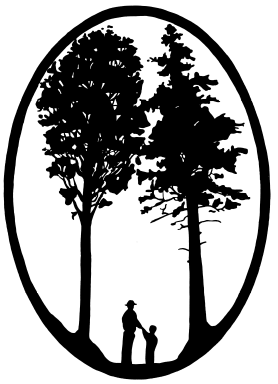
\includegraphics[width=0.3\linewidth,height=0.3\textheight]{C:/Users/Neal/projects/cruise/logo-small} 

}

\end{marginfigure}

\normalsize 

\begin{marginfigure}
\noindent \textit{\large Prepared by} 
\newline\indent Neal F. Maker and John D. Foppert  
\newline\indent Pekin Branch Forestry  
\newline\indent 1324 West County Road  
\newline\indent Calais, VT 05648  
\newline\indent (802) 229-9757  
\end{marginfigure}

\begin{marginfigure}
\noindent \textit{\large Owner}
\newline\indent Douglas Perkins Living Trust  
\newline\indent c/o Douglas Perkins

\indent 1750 Lake Dunmore Road
\newline\indent Leicester, VT 05733  
\end{marginfigure}

\begin{marginfigure}
\noindent \textit{\large Property}   
\newline\indent 27.5 acres NA   
\newline\indent Calais, VT  
\newline\indent SPAN 120-037-10679  
\newline\indent Map delineation based on VMP  
\newline\indent Photo(s) 156208, 156212, 152208, 152212  
\end{marginfigure}

\begin{marginfigure}
\noindent \textit{\large Effective date of plan}  
\newline\indent April 1, 2020  
\end{marginfigure}

\vspace{30pt} \indent This forest management plan is a blueprint for
responsible land stewardship. It is the result of a planning process
that incorporated an assessment of the history and current conditions on
the property, consideration of the various courses of future development
that the forest could follow, and discernment as to which outcomes best
suit my particular objectives.

\vspace{5pt} By signing below, I certify that I approve of---and agree
to manage my forestland according to---the following management plan. I
further certify that any of my forestland that is enrolled in Vermont's
Use Value Appraisal program is under active long-term forest management
in accordance with the state's minimum acceptable standards for forest
management. These standards include following Acceptable Management
Practices to maintain water quality on logging operations.

\vspace{38pt}

\noindent\rule{9cm}{0.4pt} \rule{.3cm}{0pt} \rule{4cm}{0.4pt}

\noindent Landowner \rule{7.7cm}{0pt} Date

\vspace{18pt}

\noindent\rule{9cm}{0.4pt} \rule{.3cm}{0pt} \rule{4cm}{0.4pt}

\noindent Landowner \rule{7.7cm}{0pt} Date

\vspace{18pt}

\noindent\rule{9cm}{0.4pt} \rule{.3cm}{0pt} \rule{4cm}{0.4pt}

\noindent Landowner \rule{7.7cm}{0pt} Date

\vspace{18pt}

\noindent\rule{9cm}{0.4pt} \rule{.3cm}{0pt} \rule{4cm}{0.4pt}

\noindent Landowner \rule{7.7cm}{0pt} Date

\vspace{24pt}

This forest management plan meets the standards promulgated by the
Vermont Department of Forests, Parks and Recreation as required for
eligibility in the Use Value Appraisal Program.

\vspace{22pt}

\noindent\rule{9cm}{0.4pt} \rule{.3cm}{0pt} \rule{4cm}{0.4pt}

\noindent County Forester \rule{7cm}{0pt} Date

\pagebreak

\section{Introduction}\label{introduction}

This plan Covers the ten year period from 2020 to 2029. It lays out the
near- and medium-term actions that should guide the development of the
Douglas Perkins Forest. It also qualifies the property for Use Value
Appraisal (UVA) and commensurate reduction in property taxes.\footnote{Further
  information about UVA and current valuations can be found at the
  Vermont Tax Department's website:
  \url{https://tax.vermont.gov/property-owners/current-use}.
  \vspace{20pt}} Owners participating in the Use Value Appraisal program
are obliged to manage their property according to the plan and to make
any reasonable investments for improvement that the plan
recommends.\footnote{UVA management plan standards are determined by the
  Department of Forests, Parks, \& Recreation and are available at
  \url{https://fpr.vermont.gov/forest/your_woods/use_value_appraisal} or
  through a County Forester.} Its recommendations were developed in
accordance with the principles and practices of scientifically sound
forestry, as described in the relevant management guidelines, textbooks
and academic journals\cite{@halligan_relative_1999}.

\section{Property Description}\label{property-description}

All of the 27.5 acre Douglas Perkins property is productive forestland
that will be managed according to this plan. Its elevations range from
1320 to 1400 feet above mean sea level. No mapped streams cross the
property, and surface waters flow to the Pekin in the south. Property
boundaries are a bit hard to find, but the corner pins have all been
located. Soils, forest health, and other pertinent topics are discussed
in the individual stand area descriptions that follow.

\section{Principles, Goals \& Strategies For Forest
Management}\label{principles-goals-strategies-for-forest-management}

\subsection{Conservation}\label{conservation}

The ecological functioning, productive capacity and biological diversity
of the forest resource should be maintained or improved over time so as
to provide opportunities for the current or future landowners to
continue to enjoy and use the property. A management strategy that is
sustainable in the long-term and viable in the short- and medium-terms
offers a strong measure of protection against future development or
conversion.

\subsection{Timber management}\label{timber-management}

Management should provide regular returns from timber harvesting.
Long-term value growth is provided by maintaining full site occupancy
with investment-grade stems: healthy trees capable of producing high
quality sawtimber or veneer and worth retaining in the stand until they
reach their full, site- and species-specific target diameters. Tree
species which yield sought-after, high-value wood should be promoted
within each stand or, when regenerating a new stand, attention should be
paid to providing the stand conditions which favor the establishment of
those species. At a property-wide scale, a variety of species should be
maintained, providing options for seizing future market opportunities
and a hedge against species-specific market depreciation. Among desired
species, additional preference should be given to individual trees of
sufficient vigor and grade-potential for strong future value growth.
Consideration of economic efficiency should inform the timing and
coordination of infrastructure investments and stand maintenance,
improvement and harvest operations.

\section{Stand Descriptions \& Management
Recommendations}\label{stand-descriptions-management-recommendations}

\begin{marginfigure} \noindent \textit{\LARGE Management Schedule} 

 \vspace{10 pt} 

 \noindent \textit{\large 2023} 

 \begin{itemize} \item Area 3: Group Selection 

 \end{itemize} \vspace{10 pt} 

 \noindent \textit{\large 2025} 

 \begin{itemize} \item Area 1: Intermediate Thinning 

 \end{itemize} \vspace{10 pt} 

 \noindent \textit{\large 2029} 

 \begin{itemize} \item Reinventory forest 

 \end{itemize} \end{marginfigure}

Presented below are detailed stand-by-stand descriptions of the forest,
the long-term structural, compositional and functional goals for each
stand, and the near-term silvicultural treatments or management
activities that have been prescribed to advance each stand toward those
goals. The data presented in the following pages was obtained from a
field examination of the property in November of 2019. General
conditions were assessed qualitatively in conjunction with quantitative
sampling. Observational notes and sample summary statistics together
provide the basis for the area descriptions and management
recommendations. All sampling was done using a systematic sample and
variable radius plots. In stands with uneven-aged structures, all trees
6" dbh and larger were measured in each plot. In stands with even-aged
structures, all main-canopy trees were measured in each plot.

When contractors are used to implement silvicultural prescriptions, they
should be highly skilled, properly equipped, fully insured, and closely
supervised. A professional forester should prepare and administer
commercial treatments, and logging operations should be timed to
coincide with favorable weather conditions (working on wet soils only
when they are frozen, for instance) and favorable timber markets. Use
Value Appraisal program guidelines allow any management activities
prescribed in this plan to be carried out up to three years before or
after the date indicated. Landowners in the Use Value Appraisal program
must file a Forest Management Activity Report with the County Forester
by February 1\textsuperscript{st} if any commercial logging occurred in
the previous year.

The property should be reinventoried in 2029 and the findings brought to
bear on a reassessment of the goals and strategies proposed in this
plan, leading to a formal management plan update. At any point over the
course of this management period, this plan may be updated to
incorporate new information and to reflect any new thoughts, concerns or
considerations on the part of the family or the foresters helping to
manage their land.

\newpage

\section{Area 1}\label{area-1}

Norway spruce\\
\noindent 5.63 legal acres \textbar{} 5.89 measured acres

\subsection{Site-specific information}\label{site-specific-information}

\begin{quote}
\begin{itemize}
\tightlist
\item
  \textbf{Soils:}\\
  \indent\indent  \textbf{Glover-Vershire complex} (shallow to
  moderately deep, excessively drained to well drained, loose, very
  rocky glacial tills on summits, shoulders, and backslopes)
\end{itemize}
\end{quote}

\begin{quote}
\begin{itemize}
\tightlist
\item
  \textbf{Site Class:}\\
  \vspace{2pt} II (determined from soil mapping and field assessment)
\end{itemize}
\end{quote}

\begin{quote}
\begin{itemize}
\tightlist
\item
  \textbf{Access:}\\
  \vspace{2pt} Good access from town road. Less than 1 mile.
\end{itemize}
\end{quote}

\begin{quote}
\begin{itemize}
\tightlist
\item
  \textbf{Stand history:}\\
  \vspace{2pt} Former pastureland, planted to Norway spruce in 1954.
  Carefully thinned by owner over the course of the last decade, though
  one section was missed and has much higher stocking (200 sq ft or so).
\end{itemize}
\end{quote}

\subsection{Current forest
information}\label{current-forest-information}

\begin{quote}
\begin{itemize}
\tightlist
\item
  \textbf{Age Class Structure:}\\
  \vspace{2pt} Even-aged\\

  \begin{marginfigure}
  \includegraphics{fmp-vt_files/figure-latex/unnamed-chunk-2-1} \caption[Distributions are approximated with kernel density estimation]{Distributions are approximated with kernel density estimation. Common species are those that account for at least 8 percent of the total stocking and areas under each curve represent species basal areas.}\label{fig:unnamed-chunk-2}
  \end{marginfigure}
\end{itemize}
\end{quote}

\begin{quote}
\begin{itemize}
\tightlist
\item
  \textbf{Species (\% stocking):}\\
  \vspace{2pt} norway spruce (92\%), white pine (8\%)
\end{itemize}
\end{quote}

\begin{quote}
\begin{itemize}
\tightlist
\item
  \textbf{Regeneration:}\\
  \vspace{2pt} Scattered patches of fir and red spruce where the
  stocking is lower.
\end{itemize}
\end{quote}

\begin{quote}
\begin{itemize}
\tightlist
\item
  \textbf{Forest health:}\\
  \vspace{2pt} A number of the Norway spruce fork at 30 or 40 ft, but
  are still healthy and pose little risk. No exotic invasive plants
  noted.
\end{itemize}
\end{quote}

\begin{quote}
\begin{itemize}
\tightlist
\item
  \textbf{Standing dead wood (sq ft/ac by size class):}\\
  \vspace{2pt} \indent \small 6-10``: 5 \textbar{} 11-16'': 0 \textbar{}
  17-22'': 0 \textbar{} 23+'': 0
\end{itemize}
\end{quote}

\subsection{Inventory information}\label{inventory-information}

\begin{quote}
\begin{itemize}
\tightlist
\item
  2 points, 10 BAF, November, 2019
\end{itemize}
\end{quote}

\begin{figure}
\includegraphics{fmp-vt_files/figure-latex/unnamed-chunk-5-1} \caption[Points represent individual plots]{Points represent individual plots. Asterisk represnts stand average. Radial lines are quadratic stand diameters.}\label{fig:unnamed-chunk-5}
\end{figure}

\begin{table}

\caption{\label{tab:unnamed-chunk-6}Measures of stocking for all live trees (Total), acceptable growing stock (AGS), and unacceptable growing stock (UGS).}
\centering
\begin{tabular}[t]{lrrr}
\toprule
Measure & Total & AGS & UGS\\
\midrule
Basal area (sq ft/ac) & 125 & 125 & 0\\
QSD (in) & 12 & 12 & NaN\\
Stems/ac & 149 & 149 & 0\\
\bottomrule
\end{tabular}
\end{table}

\begin{table}

\caption{\label{tab:unnamed-chunk-7}Current basal area (sq ft/ac) of total growing stock, acceptable growing stock, and unacceptable growing stock by size class.}
\centering
\begin{tabular}[t]{lrrr}
\toprule
Size Class & Total & AGS & UGS\\
\midrule
6-11 in. & 30 & 30 & 0\\
12-15 in. & 75 & 75 & 0\\
16-21 in. & 20 & 20 & 0\\
22+ in. & 0 & 0 & 0\\
Total & 125 & 125 & 0\\
\bottomrule
\end{tabular}
\end{table}

\subsection{Long-term management
system}\label{long-term-management-system}

\textbf{Even-Aged Management}

This stand should continue to be managed using even-aged techniques. We
recommend a rotation age of 90 or 100, which will allow for one more
thinning before regeneration is initiated (the stand is 66 now).

\subsection{Silvicultural
prescription}\label{silvicultural-prescription}

\textbf{Intermediate Thinning}\\
\noindent \textbf{Year:} 2025

The area that has not yet been thinned should be thinned, with the goal
of making it look just like the rest of the stand. Dominant and
co-dominant Norway spruce should be released and the overall stocking
should be reduced to about 140 square feet (Halligan and Nyland
\protect\hyperlink{ref-halligan_relative_1999}{1999}), which means
removing between 1/4 and 1/3 of the stocking. Note that the inventory
plots were all in spots that have already been thinned, so the
quantitative stand data does not reflect the un-thinned area.

\newpage

\section{Area 2}\label{area-2}

Mixed softwood\\
\noindent 8.22 legal acres \textbar{} 8.60 measured acres

\subsection{Site-specific
information}\label{site-specific-information-1}

\begin{quote}
\begin{itemize}
\tightlist
\item
  \textbf{Soils:}\\
  \indent\indent  \textbf{Glover-Vershire complex} (shallow to
  moderately deep, excessively drained to well drained, loose, very
  rocky glacial tills on summits, shoulders, and backslopes)
\end{itemize}
\end{quote}

\begin{quote}
\begin{itemize}
\tightlist
\item
  \textbf{Site Class:}\\
  \vspace{2pt} II -- III (determined from soil mapping and field
  assessment)
\end{itemize}
\end{quote}

\begin{quote}
\begin{itemize}
\tightlist
\item
  \textbf{Access:}\\
  \vspace{2pt} Good access from town road. Less than 1 mile.
\end{itemize}
\end{quote}

\begin{quote}
\begin{itemize}
\tightlist
\item
  \textbf{Stand history:}\\
  \vspace{2pt} Formerly pastureland, mostly planted to Norway spruce in
  1954, but establishment largely failed, probably because of thinner
  soils. No tending has been done, but many stems are are young and
  stand remains understocked.
\end{itemize}
\end{quote}

\subsection{Current forest
information}\label{current-forest-information-1}

\begin{quote}
\begin{itemize}
\tightlist
\item
  \textbf{Age Class Structure:}\\
  \vspace{2pt} Even-aged\\

  \begin{marginfigure}
  \includegraphics{fmp-vt_files/figure-latex/unnamed-chunk-8-1} \caption[Distributions are approximated with kernel density estimation]{Distributions are approximated with kernel density estimation. Common species are those that account for at least 8 percent of the total stocking and areas under each curve represent species basal areas.}\label{fig:unnamed-chunk-8}
  \end{marginfigure}
\end{itemize}
\end{quote}

\begin{quote}
\begin{itemize}
\tightlist
\item
  \textbf{Species (\% stocking):}\\
  \vspace{2pt} norway spruce (36\%), soft maple (28\%), white pine
  (16\%), fir (8\%), spruce (8\%), paper birch (4\%)
\end{itemize}
\end{quote}

\begin{quote}
\begin{itemize}
\tightlist
\item
  \textbf{Regeneration:}\\
  \vspace{2pt} Main cohort is still young.
\end{itemize}
\end{quote}

\begin{quote}
\begin{itemize}
\tightlist
\item
  \textbf{Forest health:}\\
  \vspace{2pt} Slower growth on thin soils. Many pines are poorly formed
  or infected by blister rust. No exotic invasives noted.
\end{itemize}
\end{quote}

\begin{quote}
\begin{itemize}
\tightlist
\item
  \textbf{Standing dead wood (sq ft/ac by size class):}\\
  \vspace{2pt} \indent \small 6-10``: 2.5 \textbar{} 11-16'': 0
  \textbar{} 17-22'': 0 \textbar{} 23+'': 0
\end{itemize}
\end{quote}

\subsection{Inventory information}\label{inventory-information-1}

\begin{quote}
\begin{itemize}
\tightlist
\item
  4 points, 10 BAF, November, 2019
\end{itemize}
\end{quote}

\begin{figure}
\includegraphics{fmp-vt_files/figure-latex/unnamed-chunk-11-1} \caption[Points represent individual plots]{Points represent individual plots. Asterisk represnts stand average. Radial lines are quadratic stand diameters.}\label{fig:unnamed-chunk-11}
\end{figure}

\begin{table}

\caption{\label{tab:unnamed-chunk-12}Measures of stocking for all live trees (Total), acceptable growing stock (AGS), and unacceptable growing stock (UGS).}
\centering
\begin{tabular}[t]{lrrr}
\toprule
Measure & Total & AGS & UGS\\
\midrule
Basal area (sq ft/ac) & 62 & 62 & 0\\
QSD (in) & 9 & 9 & Inf\\
Stems/ac & 143 & 143 & 0\\
\bottomrule
\end{tabular}
\end{table}

\begin{table}

\caption{\label{tab:unnamed-chunk-13}Current basal area (sq ft/ac) of total growing stock, acceptable growing stock, and unacceptable growing stock by size class.}
\centering
\begin{tabular}[t]{lrrr}
\toprule
Size Class & Total & AGS & UGS\\
\midrule
6-11 in. & 38 & 38 & 0\\
12-15 in. & 18 & 18 & 0\\
16-21 in. & 8 & 8 & 0\\
22+ in. & 0 & 0 & 0\\
Total & 62 & 62 & 0\\
\bottomrule
\end{tabular}
\end{table}

\subsection{Long-term management
system}\label{long-term-management-system-1}

\textbf{Even-Aged Management}

This stand should continue to be managed using even-aged techniques for
the time being, with a rotation age of about 110. Later in the rotation,
when more of the trees have reached commercial sizes, it may be
desirable to move the stand toward an uneven-aged structure.

\subsection{Silvicultural
prescription}\label{silvicultural-prescription-1}

No work is necessary over the next decade, but the owner may wish to do
some precommercial crop tree release to favor sapling- or pole-sized
hardwoods with good form, large crowns, and no defects. Up to 40 such
trees per acre could be released on all sides by cutting any trees with
touching crowns.

\newpage

\section{Area 3}\label{area-3}

Northern hardwood\\
\noindent 13.65 legal acres \textbar{} 14.29 measured acres

\subsection{Site-specific
information}\label{site-specific-information-2}

\begin{quote}
\begin{itemize}
\tightlist
\item
  \textbf{Soils:}\\
  \indent\indent  \textbf{Glover-Vershire complex} (shallow to
  moderately deep, excessively drained to well drained, loose, very
  rocky glacial tills on summits, shoulders, and backslopes)
\end{itemize}
\end{quote}

\begin{quote}
\begin{itemize}
\tightlist
\item
  \textbf{Site Class:}\\
  \vspace{2pt} II (determined from soil mapping and field assessment)
\end{itemize}
\end{quote}

\begin{quote}
\begin{itemize}
\tightlist
\item
  \textbf{Access:}\\
  \vspace{2pt} Pretty good through Areas 1 and 2. Less than 1 mile.
\end{itemize}
\end{quote}

\begin{quote}
\begin{itemize}
\tightlist
\item
  \textbf{Stand history:}\\
  \vspace{2pt} Current stand developed from an old sugarbush, which was
  heavily cut many years ago. Owner has begun to remove unacceptable
  growing stock and trees at risk of dying.
\end{itemize}
\end{quote}

\subsection{Current forest
information}\label{current-forest-information-2}

\begin{quote}
\begin{itemize}
\tightlist
\item
  \textbf{Age Class Structure:}\\
  \vspace{2pt} Even-aged\\

  \begin{marginfigure}
  \includegraphics{fmp-vt_files/figure-latex/unnamed-chunk-14-1} \caption[Distributions are approximated with kernel density estimation]{Distributions are approximated with kernel density estimation. Common species are those that account for at least 8 percent of the total stocking and areas under each curve represent species basal areas.}\label{fig:unnamed-chunk-14}
  \end{marginfigure}
\end{itemize}
\end{quote}

\begin{quote}
\begin{itemize}
\tightlist
\item
  \textbf{Species (\% stocking):}\\
  \vspace{2pt} hard maple (40\%), beech (17\%), black cherry (11\%),
  paper birch (11\%), ash (6\%), soft maple (6\%), yellow birch (6\%),
  hophornbeam (2\%)
\end{itemize}
\end{quote}

\begin{quote}
\begin{itemize}
\tightlist
\item
  \textbf{Regeneration:}\\
  \vspace{2pt} Dominated by diseased beech suckers.
\end{itemize}
\end{quote}

\begin{quote}
\begin{itemize}
\tightlist
\item
  \textbf{Forest health:}\\
  \vspace{2pt} Deer browse and suckering of diseased beech stems is
  impeding the regeneration of desirable species. Many of the overstory
  sugar maples are experiencing crow dieback. No exotic invasives noted.
\end{itemize}
\end{quote}

\begin{quote}
\begin{itemize}
\tightlist
\item
  \textbf{Standing dead wood (sq ft/ac by size class):}\\
  \vspace{2pt} \indent \small 6-10``: 1.7 \textbar{} 11-16'': 0
  \textbar{} 17-22'': 1.7 \textbar{} 23+'': 0
\end{itemize}
\end{quote}

\subsection{Inventory information}\label{inventory-information-2}

\begin{quote}
\begin{itemize}
\tightlist
\item
  6 points, 10 BAF, November, 2019
\end{itemize}
\end{quote}

\begin{figure}
\includegraphics{fmp-vt_files/figure-latex/unnamed-chunk-17-1} \caption[Points represent individual plots]{Points represent individual plots. Asterisk represnts stand average. Radial lines are quadratic stand diameters.}\label{fig:unnamed-chunk-17}
\end{figure}

\begin{table}

\caption{\label{tab:unnamed-chunk-18}Measures of stocking for all live trees (Total), acceptable growing stock (AGS), and unacceptable growing stock (UGS).}
\centering
\begin{tabular}[t]{lrrr}
\toprule
Measure & Total & AGS & UGS\\
\midrule
Basal area (sq ft/ac) & 78 & 63 & 15\\
QSD (in) & 11 & 12 & 9\\
Stems/ac & 114 & 80 & 34\\
\bottomrule
\end{tabular}
\end{table}

\begin{table}

\caption{\label{tab:unnamed-chunk-19}Current basal area (sq ft/ac) of total growing stock, acceptable growing stock, and unacceptable growing stock by size class.}
\centering
\begin{tabular}[t]{lrrr}
\toprule
Size Class & Total & AGS & UGS\\
\midrule
6-11 in. & 25 & 15 & 10\\
12-15 in. & 48 & 45 & 3\\
16-21 in. & 5 & 3 & 2\\
22+ in. & 0 & 0 & 0\\
Total & 78 & 63 & 15\\
\bottomrule
\end{tabular}
\end{table}

\subsection{Long-term management
system}\label{long-term-management-system-2}

\textbf{Selection System}

The stand should be converted to an uneven-aged structure (R. D. Nyland
\protect\hyperlink{ref-nyland_even-_2003}{2003}), which will allow the
owners to keep working with the valuable trees that are present now,
while regenerating areas with little potential value growth. Eventually
we will establish a system with harvests about every 10 years, which
will remove mature trees, release immature trees, and establish or
release new regeneration. Target diameters for crop trees will be
specific to individual species as follows: 24 inches for sugar maple,
yellow birch, and black cherry; and 18 inches for other commercial
hardwoods (with exceptions allowed for all veneer quality hardwood
stems).

\subsection{Silvicultural
prescription}\label{silvicultural-prescription-2}

\textbf{Group Selection}\\
\noindent \textbf{Year:} 2023

This treatment will begin the process of converting the stand to an
uneven-aged structure using group selection; which R. D. Nyland
(\protect\hyperlink{ref-nyland_even-_2003}{2003}) refers to as a ``patch
cutting conversion strategy''. Groups of trees should be harvested to
create openings in the canopy and allow for the establishment of
desirable regeneration. These groups openings should be from 1/10 to one
acre in size (about 35 to 100 feet in diameter), and should be located
to remove concentrations of unacceptable growing stock, trees with
severe crown dieback, and sawtimber size ash (which have a very high
risk of dying from emerald ash borer infestation in the next decade).
The group openings are preferable to Nyland's ``uniform cutting
conversion strategies'' because they have a better chance of overcoming
diseased beech and securing regeneration of other species, but in order
for them to be successful, all beech need to be removed from them,
including saplings. If any saplings of desirable species are found in
the openings, they should be kept and protected from damage. Desirable
species that should be favored include sugar maple, yellow birch, black
cherry, red maple, and paper birch. These are also the species we hope
to regenerate. Overall, group openings should not cover any more than
1/3rd of the whole stand area. \par Outside of and between openings, a
light thinning should be carried out to remove unacceptable growing
stock and sawtimber sized ash while maintaining full stocking. The basal
area outside openings should not be reduced below about 70 square feet
per acre (b-line; Leak, Solomon, and DeBald
\protect\hyperlink{ref-leak_silvicultural_1987}{1987}). This will help
to keep the beech problem in check.\footnote{Above b-line, overstory
  trees should provide enough shade to prevent additional beech root
  suckering. Meanwhile, the high-light conditions inside the group
  openings should allow other species to out-compete the beech suckers
  there. The beeches become a problem at intermediate stocking levels,
  where they get some light while remaining competitive.}

\newpage

\section*{References}\label{references}
\addcontentsline{toc}{section}{References}

\hypertarget{refs}{}
\hypertarget{ref-halligan_relative_1999}{}
Halligan, J. P., and R. D. Nyland. 1999. ``Relative Density Guide for
Norway Spruce Plantations in Central New York.'' \emph{Northern Journal
of Applied Forestry} 16 (3): 154--59.
doi:\href{https://doi.org/10.1093/njaf/16.3.154}{10.1093/njaf/16.3.154}.

\hypertarget{ref-leak_silvicultural_1987}{}
Leak, William B., Dale S. Solomon, and Paul S. DeBald. 1987.
``Silvicultural Guide for Northern Hardwood Types in the Northeast
(Revised).'' Research paper NE-603. U.S. Department of Agriculture,
Forest Service, Northeastern Forest Experiment Station.

\hypertarget{ref-nyland_even-_2003}{}
Nyland, Ralph D. 2003. ``Even- to Uneven-Aged: The Challenges of
Conversion.'' \emph{Forest Ecology and Management} 172 (2-3): 291--300.
doi:\href{https://doi.org/10.1016/S0378-1127(01)00797-6}{10.1016/S0378-1127(01)00797-6}.



\end{document}
